%%%%%%%% ICML 2020 EXAMPLE LATEX SUBMISSION FILE %%%%%%%%%%%%%%%%%

\documentclass{article}

% Recommended, but optional, packages for figures and better typesetting:
\usepackage{microtype}
\usepackage{graphicx}
\usepackage{subfigure}
\usepackage{booktabs} % for professional tables

% hyperref makes hyperlinks in the resulting PDF.
% If your build breaks (sometimes temporarily if a hyperlink spans a page)
% please comment out the following usepackage line and replace
% \usepackage{icml2020} with \usepackage[nohyperref]{icml2020} above.
\usepackage{hyperref}

% Attempt to make hyperref and algorithmic work together better:
\newcommand{\theHalgorithm}{\arabic{algorithm}}

% Use the following line for the initial blind version submitted for review:
% \usepackage{icml2020}

% If accepted, instead use the following line for the camera-ready submission:
\usepackage[accepted]{icml2020}

\usepackage{mathtools}
\usepackage{amsmath}
\usepackage{amssymb}

% The \icmltitle you define below is probably too long as a header.
% Therefore, a short form for the running title is supplied here:
\icmltitlerunning{Solving Lunar Lander with a DQN}

\begin{document}

\twocolumn[
\icmltitle{Solving Lunar Lander with a DQN}

% It is OKAY to include author information, even for blind
% submissions: the style file will automatically remove it for you
% unless you've provided the [accepted] option to the icml2020
% package.

% List of affiliations: The first argument should be a (short)
% identifier you will use later to specify author affiliations
% Academic affiliations should list Department, University, City, Region, Country
% Industry affiliations should list Company, City, Region, Country

% You can specify symbols, otherwise they are numbered in order.
% Ideally, you should not use this facility. Affiliations will be numbered
% in order of appearance and this is the preferred way.
% \icmlsetsymbol{equal}{*}

\begin{icmlauthorlist}
\icmlauthor{Frederik J. Mellbye}{to}
\end{icmlauthorlist}

\icmlaffiliation{to}{Institute for Computational and Mathematical Engineering, Stanford University, Stanford, USA}

\icmlcorrespondingauthor{Frederik J. Mellbye}{frederme@stanford.edu}

% You may provide any keywords that you
% find helpful for describing your paper; these are used to populate
% the "keywords" metadata in the PDF but will not be shown in the document
\icmlkeywords{Machine Learning, ICML}

\vskip 0.3in
]

% this must go after the closing bracket ] following \twocolumn[ ...

% This command actually creates the footnote in the first column
% listing the affiliations and the copyright notice.
% The command takes one argument, which is text to display at the start of the footnote.
% The \icmlEqualContribution command is standard text for equal contribution.
% Remove it (just {}) if you do not need this facility.

\printAffiliationsAndNotice{}  % leave blank if no need to mention equal contribution
% \printAffiliationsAndNotice{\icmlEqualContribution} % otherwise use the standard text.

\begin{abstract}
A DQN is employed to solve the game Lunar Lander. The artificial neural network architecture is tuned over various learning rates and optimizers. The DQN agent successfully solves the game after around 1000 episodes of playing the game.
\end{abstract}

\section{Introduction}
\label{introduction}

Playing games has been one of the great successes of Reinforcement Learning (RL). Most notably, human level play has been acheived in a large number of different Atari games \cite{mnih2015humanlevel}. This project applies similar methodology to the game Lunar Lander.

Lunar Lander is a simple 2D control environment available in OpenAI gym \cite{gym}. The goal is to successfully land a lander on a target pad, always located at the origin. See Figure~\ref{fig:screenshot} for the game interface.

At each time step $t$, the current state is revealed to the agent playing the game. It is given by
\begin{align}
  s_t = \begin{bmatrix} x & y & v_x & v_y & \phi & \omega & l_1 & l_ 2 \end{bmatrix}
\end{align}
where $(x,y)$ is the position, $(v_x, v_y)$ is the velocity, $\phi$ is the angle of rotation, $\omega$ is the angular velocity and $l_1, l_2 \in \{ 0,1 \}$ indicate whether the left and right legs are touching the surface.

Four actions are available at each time step: do nothing, fire left engine, fire right engine and fire main thruster. The action chosen at each time step is denoted $a_t$. Once an action is chosen the game progresses, and reveals a reward $r_t$ and the next state $s_{t+1}$.

The total reward from moving from the top to the landing pad is usually in the range $100 - 140$, with points deducted if the lander at a given time step moves away from the landing pad. The episode finishes if the lander comes to rest (lands) or crashes, which gives an additional reward of $100$ or $-100$. Leg contact with the ground is $+10$. Firing the main engine is $-0.3$ points. Solving the game, i.e. successfully landing between the flags, grants a reward of 200. The reward at each time step is denoted $r_t$.

In many nonlinear control applications the dynamics are nonlinear and challenging to model. Traditional control system theory (MPC is commonly used) often relies on such models, which in some cases is a drawback. Another drawback is the need to solve the optimal control problem on-line, which can be too time consuming. On certain problems it has been shown that RL may be competitive with MPC, even in contexts where a good system model is available \cite{control}. It is therefore of interest to develop an understanding of how RL approaches can be applied to such problems.

\begin{figure}
  \includegraphics[width=\linewidth]{images/screenshot.png}
  \caption{Screenshot from the Lunar Lander game.}
  \label{fig:screenshot}
\end{figure}

\section{Background}
\label{background}
This section walks through some of the basics of Deep Q-learning that were used to acheive human level play in Atari games.

\subsection{Reinforcement learning}

\subsection{Deep Q-learning}
The Q-learning algorithm \cite{watkins} was one of the early breakthroughs of Reinforcement Learning. Defined by
\begin{align}
  \label{eq:Qlearning}
  Q(s_t, a_t) \gets Q(s_t, a_t) + \alpha \Big[ r_t + \gamma \max_a Q(s_t, a) - Q(s_t, a_t)\Big]
\end{align}
Q-learning learns $Q$, which approximates the optimal action-value function $q^*$.

In most applications a tabular representation of $Q(s,a) \forall s \in \mathcal{S}, a \in \mathcal{A}$ is infeasible. Instead a function approximator is commonly used. An important case

Artificial neural networks (ANNs) are commonly used for nonlinear function approximation. In Deep Q-learning a neural network $Q$ approximates the action value function \cite{Sutton1998}, in that for a given state $s$ it outputs a vector of action values $Q(s,\cdot; \theta)$.

Since $Q$ maps state-action pairs to estimates of their values, a straight forward approach is to have the neural network take the state and action as input. An issue with this approach is that a separate forward pass is required to compute the value for each action. A more efficient approach uses an architecture with one output for each possible action, since only one forward pass is required to compute values for all actions \cite{mnih2015humanlevel}.

A fundamental aspect of Reinforcement Learning is the tradeoff of exploration and exploitation. To ensure adequate exploration $\epsilon$-greedy is commonly used: Take a random action with probability $\epsilon$
and the greedy action $\underset{a}{\arg \max} Q(s,a)$ otherwise. This gives the policy
\begin{align*}
  \pi_\theta (s) =
  \begin{cases}
    \text{random}                   & \text{with probability } \epsilon \\
    \underset{a}{\arg \max} Q(s, a) & \text{otherwise}
  \end{cases}
\end{align*}

\subsection{Double DQN}
Lunar Lander is a stochastic environment. Each episode has different moon surfaces, landing pad angles and importantly, the lander spawns with different initial translational and rotational positions and velocities.

In such environments, vanilla Q-learning commonly performs pooly due to large overestimations of action values. These overestimations result from inherent bias in Q-learning, the same value is used both to select and evaluate an action. In a particular state, actions with overestimated values are thus more likely to be picked and evaluated favorably.

Double Q-learning maintains two value functions $\theta$ and $\theta'$, where $\theta$ is used for selecting actions and the $\theta'$ to evaluate those actions. This addresses the issue of maximization bias. Each experience is randomly assigned to update one of the value functions. The double Q-learning target is therefore
\begin{align*}
  R_{t+1} + \gamma Q(S_{t+1}, \arg \max_a Q(S_{t+1}, a; \theta_t); \theta'_t)
\end{align*}
The idea of double Q-learing can be applied to the DQN setting \cite{Hasselt2016DeepRL}. The evaluation network $\theta'$ is replaced by a target network $\theta^{-}$, a periodic copy of the online weights $\theta$. The target is therefore
\begin{align*}
  R_{t+1} + \gamma Q(S_{t+1}, \arg \max_a Q(S_{t+1}, a; \theta_t); \theta_t^{-})
\end{align*}
The target network is updated every $C$ iterations. This is known as Double DQN. Using a target network is also crucial for stability of training in stochastic environments.

\subsection{Experience replay}
Training neural networks commonly requires large amounts of data, here this corresponds to many experienced $(s,a,r,s')$ tuples. In experience replay, a buffer $\mathcal{D}$ of fixed size is used to hold experiences. In each time step a minibatch of experiences are sampled unformly with replacement from the buffer and used for training the network.

\section{Approach}
\label{approach}
In this project the approach follows closely \cite{Mnih2013PlayingAW}, with a minor simplification, namely that the states are not given by the pixel values on the screen. There is thus no need for convolutional layers in the architecture.

The approach is described in detail in the following subsections and summarized in Algorithm~\ref{alg:ddqn}. The parameter values that were used to successfully solve the game are shown in Table~\ref{tbl:params}.

The parameter values used in \cite{mnih2015humanlevel} were first used as a baseline, and then tuned for better performance in the Lunar Lander environment.

\begin{figure}
  \centering
  \includegraphics[width=.6\linewidth]{images/architecture.png}
  \caption{DQN architecture visualized, with fewer neurons per hidden layer than what is used in the project. Created using \url{http://alexlenail.me/NN-SVG/index.html}.}
  \label{fig:archi}
\end{figure}

\subsection{DQN architecture}
Several neural network architectures are explored, varying the size and number of hidden layers. The function approximation needs to be sufficiently flexible to learn all the required behaviours: hovering, steering back towards the landing pad and carefully landing. However, if the network is too flexible (high variance), training will be unstable or require too large amounts of data. As in \cite{mnih2015humanlevel} ReLu activation is used for the hidden layers. The output layer has linear activation, since $Q(s,a) \in \mathbb{R}$.

Experimentation was also performed with varying the learning rate and optimizer. Adam and Stochastic Gradient Descent (SGD) is compared with RMSProp, which was used in \cite{mnih2015humanlevel}.

\subsection{Reinforcement learning}

The value of discount factor $\gamma$ is important, as it essentially choses whether to prioritize short term or long term rewards. Here $\gamma = 0.99$ is used, which is the same as in \cite{mnih2015humanlevel}. This gives adequate long term weight such that the agent learns that more reward is possible when it gets close to the landing pad.

In this project the exploration rate is linearly annealed from an initial exploration rate $\epsilon_0$ to $\epsilon_\text{final}$ over the course of $n_\epsilon$ episodes. The exploration is then kept at $\epsilon_\text{final}$.

\subsection{Correctness verification}
To verify the correctness of the implementation, there should be a clear positive trend in the average reward and the agent should eventually successfully land. An average reward of over $200$ indicates that the agent is very successful at landing with some failures.

\begin{algorithm}[tb]
   \caption{Double DQN.}
   \label{alg:ddqn}
\begin{algorithmic}[1]
  \FOR{$\text{episode} = 1, \hdots, M$}
    \STATE Observe $s_1$
    \FOR{$t = 1, \hdots, T$}
      \STATE Select action
      \begin{align*}
        a_t = \begin{cases}
          \text{Random} & \text{with probability } \epsilon \\
          \underset{a}{\arg \max} Q(s_t, a; \theta) & \text{otherwise}
        \end{cases}
      \end{align*}
      \STATE Perform action $a_t$ and observe $r_t$ and $s_{t+1}$
      \STATE Store experience tuple $(s_{t}, a_{t}, r_{t}, s_{t+1})$ in $\mathcal{D}$
      \STATE Sample random minibatch of transitions $(s_j, a_j, r_j, s_{j+1})$
      \STATE Set targets $y_j = $
      \begin{align*}
        \begin{cases}
          r_j & \text{if } s_{t+1} \text{ terminal} \\
          r_j + \gamma \max_{a'} Q(s_{j+1}, a'; \theta^{-}) & \text{otherwise}
        \end{cases}
      \end{align*}
      \STATE Perform one pass of gradient descent over the minibatch with loss $(y_j - Q(s_j, a_j; \theta))^2$ w.r.t. $\theta$
      \STATE Reset $\theta^{-} = \theta$ every $C$ steps.
    \ENDFOR
  \ENDFOR
\end{algorithmic}
\end{algorithm}

\begin{table*}[t]
  \centering
  \caption{Parameters used to solve Lunar Lander.}
  \label{tbl:params}
\begin{tabular}{*4l} \toprule
\emph{Name}       & \emph{Symbol} & \emph{Value} & \emph{Description} \\ \midrule
Max episode length                 & $T$ & 400 & \\
Discount factor & $\gamma$ & 0.99   & \\
Minibatch size &  & 64 & \\
Replay buffer size & & 100000 & Number of ($s,a,r,s'$) tuples stored in $\mathcal{D}$ \\
Episodes before updates & & 20 & Episodes with uniform policy before training \\
Target network update period & $C$ & 1000 & Update $\theta^{-} := \theta$ every $C$ iterations \\
Optimizer & & Adam & As implemented in \texttt{tf.keras} \\
Learning rate & $\eta$ & 0.0002 & \\
Hidden layer sizes & & 256, 128 & \\
Initial exploration & $\epsilon_0$ & 1.0 & \\
Final exploration & $\epsilon_{\text{final}}$ & 0.01 & \\
Final exploration episode & $n_\epsilon$ & 1000 & Episodes with linearly decaying exploration \\ \bottomrule
\end{tabular}
\end{table*}

\section{Results}
\label{results}
Figure~\ref{fig:lr} shows the mean reward after 200 episodes with different learning rates and optimizers. We see that ...

\begin{figure}[tb]
  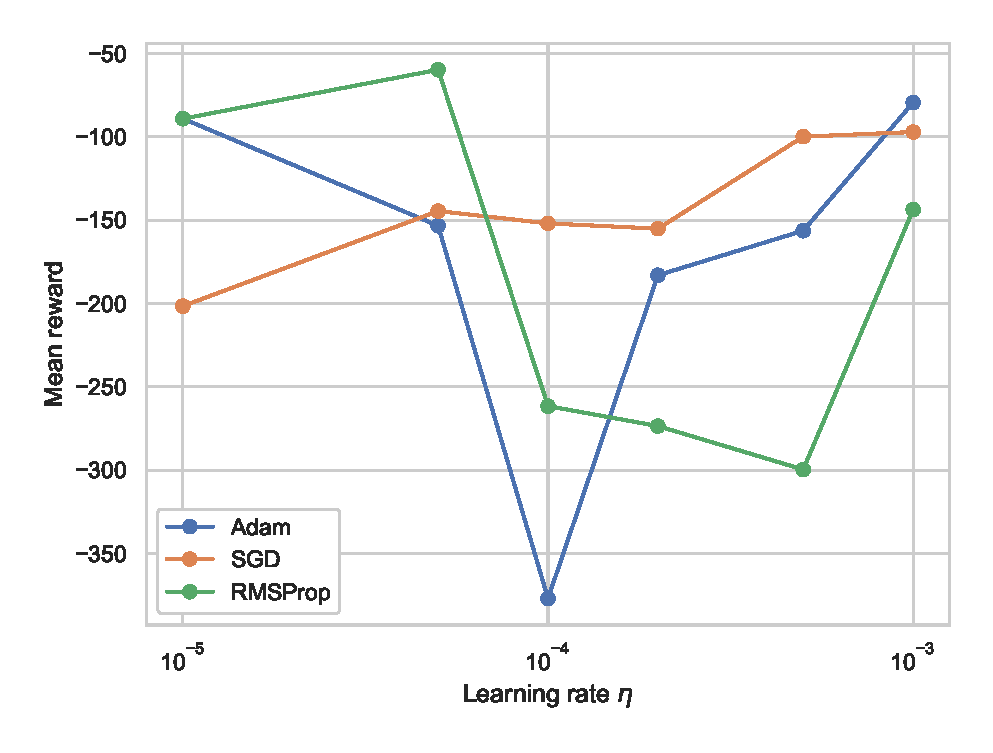
\includegraphics[width=\linewidth]{figures/learning_rate.eps}
  \caption{Mean reward after 200 episodes of training for different learning rates and optimizers. The mean of the last 100 episodes is used. RMSProp used the default $\rho = 0.9$.}
  \label{fig:lr}
\end{figure}

Figure~\ref{fig:training} shows 1500 episodes of training with the setup shown in Table~\ref{tbl:params}. We see that the agent steadily improves over the course of training before plateauing around a mean reward slightly above 200.

\begin{figure}[tb]
  \centering
  \includegraphics[width=\linewidth]{figures/long_training.pdf}
  \caption{Reward for each episode of training (blue) and the mean reward of the last 100 episodes (orange). The agent steadily improves until it plateaus slightly above a total reward of 200. This training sequence used the parameters listed in Table~\ref{tbl:params}.}
  \label{fig:training}
\end{figure}

Multiple neural network architectures were tried and evaluated heuristically. A single hidden layer network acheived no improvement and had performance similar to a random agent, indicating that there is too much bias. With three hidden layers the play was also indistinguishable from that of a random agent, indicating too large model variance. The hidden layer sizes were increased as powers of two until the model succesfully improved as it saw more data. This behavior very clearly occured with two hidden layers with 256 and 128 neurons respectively, so this was chosen as the architecture.

The DQN agent discovers different skills as the training progresses. First, it learns to hover and gradually to stabilize and turn back towards the center. It then learns to slowly descend towards the ground, but for a long time does not discover that it needs to stop firing the engines and come to a complete halt to land.

Notice the large amount of variation in total reward per episode. In some episodes, even towards the end, the lander crashes. From watching these episodes the crashes seem to appear when there is large initial $|v_x|$ and a steep hill. In these cases the lander does not steer towards the center sufficiently quickly and crashes violently, suggesting that further improvement is possible.

\section{Conclusion}
\label{conclusion}
A setup is found such that the agent plays the game very successfully.

Neural network architecture important. Too simple: Insufficient complexity in representation of all actions, too complex: Training too slow/not stable.

\section{Future directions}
Many possible improvements are available in the literature. I believe using prioritized experience replay seems very interesting, since some states and action are more important than others \cite{Schaul2016PrioritizedER}. In particular, as an example, the lander spent a long time to learn to apply the action "no thrust" to finally land. When this occurs due to exploration the large instant reward of +200 gives a large estimated TD error. In prioritized experience replay we would sample this experience more frequently and hopefully learn the final part of landing faster.

Another possible improvement is to actually use Double Q-learning, with two separate Q-networks parametrized by $\theta$ and $\theta'$. This could accellerate training as there could still be maximization bias with the target network.

Finally, future work should perform more extensive tuning of the current setup to decrease the number of episodes/updates required to solve the game. Neural network structures could be explored more extensively and rigorously. Additionaly other tweaks could be attempted, such as adding momentum to the solvers.


% In the unusual situation where you want a paper to appear in the
% references without citing it in the main text, use \nocite

\bibliography{references}
\bibliographystyle{icml2020}

%%%%%%%%%%%%%%%%%%%%%%%%%%%%%%%%%%%%%%%%%%%%%%%%%%%%%%%%%%%%%%%%%%%%%%%%%%%%%%%
%%%%%%%%%%%%%%%%%%%%%%%%%%%%%%%%%%%%%%%%%%%%%%%%%%%%%%%%%%%%%%%%%%%%%%%%%%%%%%%


\end{document}


% This document was modified from the file originally made available by
% Pat Langley and Andrea Danyluk for ICML-2K. This version was created
% by Iain Murray in 2018, and modified by Alexandre Bouchard in
% 2019 and 2020. Previous contributors include Dan Roy, Lise Getoor and Tobias
% Scheffer, which was slightly modified from the 2010 version by
% Thorsten Joachims & Johannes Fuernkranz, slightly modified from the
% 2009 version by Kiri Wagstaff and Sam Roweis's 2008 version, which is
% slightly modified from Prasad Tadepalli's 2007 version which is a
% lightly changed version of the previous year's version by Andrew
% Moore, which was in turn edited from those of Kristian Kersting and
% Codrina Lauth. Alex Smola contributed to the algorithmic style files.
